\begin{tabular}{lp{2.5in}}
\raisebox{.3in}{
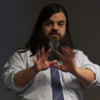
\includegraphics{../pictures/Bryan.jpg}} &
\raisebox{1in}{\parbox{2.4in}{\textbf{Bryan Alexander --- USA, VT (Author)} I research the ways new
technologies change education, teaching, learning, and scholarship. I'm
passionate about storytelling, gaming, pedagogy, and understanding the
future. My family homesteads on top of a little mountain, raising
food.
% \href{https://twitter.com/\#!/BryanAlexander}{Bryan on
%Twitter} \textbar{} \href{http://bryanalexander.org/}{Bryan's personal
%website}
}}
\end{tabular}

\marktransitionempty

\begin{tabular}{lp{2.5in}}
\raisebox{.3in}{

\includegraphics{../pictures/Paul.jpg}
} &
\raisebox{1in}{\parbox{2.4in}{\textbf{Paul Allison --- USA, NY (Author)} Currently,
I teach English at the \href{http://bronxbash.com}{Bronx Academy Senior
High}. Another community that I'm a part of is the
\href{http://nycwritingproject.org}{New York City Writing Project}. I'm
the NYC Technology Liaison for the \href{http://nwp.org}{National
Writing Project}. I help to manage
\href{http://youthvoices.net\%20}{Youth Voices} and I co-produce
\href{http://teachersteachingteachers.org}{Teachers Teaching
Teachers}.
%\href{https://plus.google.com/u/0/113993022447291199374/about}{Paul on
%Google+} \textbar{} \href{http://teachersteachingteachers.org}{Paul's
%personal website}\href{http://teachersteachingteachers.org}{}
}}
\end{tabular}

\newpage
\marktransitionempty

\begin{tabular}{lp{2.5in}}
\raisebox{.3in}{
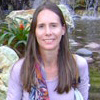
\includegraphics{../pictures/Maria.jpg}
} &
\raisebox{1in}{\parbox{2.4in}{\textbf{Mar\'ia F. Arenas --- República Argentina} \textbf{(Author, Editor)} Independent consultant researcher on TICS applied to
Learning, Digital Communication, Institutional, Corporate. On line
facilitator tutorship. Professor on Semiotics, Social Communication,
Networking. 
%\href{https://plus.google.com/u/0/stream/circles/p2e54657d0d6fc86d}{Mar\'ia
%on Google+} \textbar{} \textbf{
%}\href{http://arenastudies.wordpress.com/}{Mar\'ia's personal website}
}}
\end{tabular}

\marktransitionempty

\begin{tabular}{lp{2.5in}}
\raisebox{.3in}{
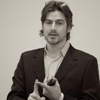
\includegraphics{../pictures/Regis.jpg}
} &
\raisebox{1in}{\parbox{2.4in}{\textbf{R\'egis Barondeau --- Canada} \textbf{(Author)} I build bridges between
research, praxeology and technology and I become creative ``by finding a
likeness between things which were not thought alike before''
(Bronowski, 1958). I'm interested in complexity, culture, social media
especially wikis, education, open government and more.
%Reach \href{https://twitter.com/regisbarondeau}{R\'egis on Twitter}
%\textbar{} \href{http://www.regisbarondeau.com}{Regis' personal website}
}}
\end{tabular}

\marktransitionempty

\begin{tabular}{lp{2.5in}}
\raisebox{.5in}{
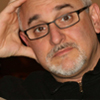
\includegraphics{../pictures/Doug.jpg}
} &
\raisebox{1.2in}{\parbox{2.4in}{\textbf{Doug Breitbart --- USA, NJ (Author, Meeting Support)} I a
catalyst and provocateur who has worn the hats of attorney, consultant,
facilitator, coach, entrepreneur, father, husband, student, teacher.
%\href{http://www.linkedin.com/profile/view?id=791427\&trk=tab\_pro}{Doug
%on LinkedIn} \textbar{} \href{www.ontologique.com}{Doug's personal
%website}
}}
\end{tabular}

\marktransitionempty

\begin{tabular}{lp{2.5in}}
\raisebox{.3in}{
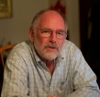
\includegraphics{../pictures/George.jpg}
} &
\raisebox{1in}{\parbox{2.4in}{\textbf{George Brett --- USA, VAN (Author, Edior, Meeting Support)} Twitter Bio: “autodidactic techno arsty craftsy eclecticist.” Many years as a diplomat for IT technology as applied to research and education. I’m a teacher/trainer, consultant, analyst, info ferret, artist, life-long learner, and member of a great family. Current challenges include: best way to share skills and experiences with others and as a Gen-Boomer finding more steady work.
%\href{http://www.linkedin.com/in/ghbrett/}{George on LinkedIn} \textbar{} \href{http://ghbrett.org/}{George's personal website}
}}
\end{tabular}

\marktransitionempty

\begin{tabular}{lp{2.5in}}
\raisebox{.3in}{
\includegraphics{../pictures/Suz.jpg}}
&
\raisebox{1in}{\parbox{2.4in}{\textbf{Suz Burroughs - USA, CA} \textbf{(Author, Designer)} I enable the connections between the teacher and learner in all of us by designing robust, measurable learning environments where people share their knowledge and experience with each other. Learning Designer, Design Thinking facilitator, Visiting Professor of Innovation.
%\href{http://susanburroughs.squarespace.com/}{Suz' personal website}
}}
\end{tabular}

\marktransitionempty

\begin{tabular}{lp{2.5in}}
\raisebox{.3in}{
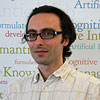
\includegraphics{../pictures/Joe.jpg}
} &
\raisebox{1in}{\parbox{2.4in}{\textbf{Joe Corneli --- U.K.} \textbf{(Author, Editor)} Joe Corneli does research on the anthropology of modern mathematics. He is a member
of the board of directors of the US-based nonprofit, PlanetMath.org,
and a research student at the Knowledge Media Institute of The Open
University, UK.
%Reach \href{http://identi.ca/arided}{Joe on Identi.ca}
%\textbar{} \href{http://metameso.org/~joe}{Joe's personal website}
}}
\end{tabular}


\marktransitionempty

\begin{tabular}{lp{2.5in}}
\raisebox{.3in}{
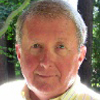
\includegraphics{../pictures/Jay.jpg}
} &
\raisebox{1in}{\parbox{2.4in}{\textbf{Jay Cross --- USA, CA} \textbf{(Author)} Jay is the Johnny Appleseed of informal learning. The \href{http://internettimealliance.com/}{Internet Time Alliance}, which he chairs, helps corporations and governments use networks to accelerate performance.
%\href{mailto:jaycross@internettime.com}{Jay by email} \textbar{}
%\href{http://jaycross.com/}{Jay's personal website}
}}
\end{tabular}

\marktransitionempty

\begin{tabular}{lp{2.5in}}
\raisebox{.3in}{
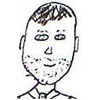
\includegraphics{../pictures/Charlie.jpg}
} &
\raisebox{1in}{\parbox{2.4in}{\textbf{Charles Jeffrey Danoff --- USA, IL} \textbf{(Author)} Charles is the Owner of Mr.
Danoff's Teaching Laboratory, an Educational Publishing and Services
firm he established in 2009.  He started co-publishing
research on Paragogy, Peeragogy's inspiration, in late 2010.
%\href{http://identi.ca/mrd}{Charles on Identi.ca} \textbar{}
%\href{http://mr.danoff.org}{Charles' personal website}
}}
\end{tabular}

\marktransitionempty

\begin{tabular}{lp{2.5in}}
\raisebox{.3in}{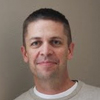
\includegraphics{../pictures/James.jpg}}
&
\raisebox{1in}{\parbox{2.4in}{\textbf{James Folkestad - USA, CO (Author, Editor, Designer, Developer)} My approach to
education has shifted from an emphasis on my teaching, to a more central
focus on student learning, and finally to an activity-systems approach
as I have come to realize that the two (teacher and learner) are
inseparable parts of the learning ecosystem. 
%Reach
%\href{https://plus.google.com/u/0/114552232610071440407/about}{James on
%Google+} \textbar{} \href{http://edgility.net}{James' personal
%website} 
}}
\end{tabular}

\marktransitionempty

\begin{tabular}{lp{2.5in}}
\raisebox{.3in}{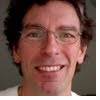
\includegraphics{../pictures/John.jpg}}
&
\raisebox{.8in}{\parbox{2.4in}{\textbf{John Graves - Australia (Editor)} 

Founder of SlideSpeech. Graduate of Singularity University. \medskip

%Reach \href{http://twitter.com/slidespeech}{John on Twitter} \textbar{} \href{http://slidespeech.tumblr.com/}{John's personal website} }}\\
}}
\end{tabular}

\marktransitionempty

\begin{tabular}{lp{2.5in}}
\raisebox{.3in}{
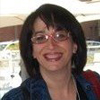
\includegraphics{../pictures/Gigi.jpg}
} &
\raisebox{1in}{\parbox{2.4in}{\textbf{Gigi Johnson, EdD --- USA, CA (Author, Developer)} I mix formal learning
programs with programs to help learners begin to work, live, and create
everywhere. My own adventures include writing, singing, video, teaching,
and parenting 3 teens.
%\href{http://twitter.com/maremel}{Gigi on
%Twitter} \textbar{} \href{http://maremel.com}{Gigi's personal
%page}
}}
\end{tabular}

\marktransitionempty

\begin{tabular}{lp{2.5in}}
\raisebox{.3in}{
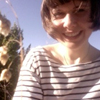
\includegraphics{../pictures/Anna.jpg}
} &
\raisebox{1in}{\parbox{2.4in}{\textbf{Anna Keune --- Germany/Finland} \textbf{(Co-author, Designer)} I design technology for learning and I like it.  I'm affiliated with the Media Lab Helsinki, Aalto University School of Arts, Design and Architecture.
%\href{https://twitter.com/\#!/akeune}{Anna on Twitter} \textbar{}
%\href{http://www.annakeune.com}{Anna's personal website}
}}
\end{tabular}

\marktransitionempty

\begin{tabular}{lp{2.5in}}
\raisebox{.3in}{
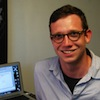
\includegraphics{../pictures/Kyle.jpg}
} &
\raisebox{1in}{\parbox{2.4in}{\textbf{Kyle Larson --- FL, USA (Editor)} 
Kyle Larson is an undergraduate thesis student at New College of Florida. His research interests include composition theory, rhetorical theory, computers and composition, and pedagogy.
%\href{https://plus.google.com/110988036495982155492/posts}{Kyle on Google+}
}}
\end{tabular}

\marktransitionempty

\begin{tabular}{lp{2.5in}}
\raisebox{.3in}{
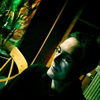
\includegraphics{../pictures/Roland.jpg}
} &
\raisebox{1in}{\parbox{2.4in}{\textbf{Roland Legrand --- Belgium (Author)} I'm a financial journalist, heavily
involved in experimenting with social media and new forms for reporting
and community conversation.
%\href{http://www.twitter.com/rolandlegrand}{Roland on Twitter}
%\textbar{} \href{http://www.mixedrealities.com}{Roland's personal
%website}
}}
\end{tabular}

\marktransitionempty

\begin{tabular}{lp{2.5in}}
\raisebox{.3in}{
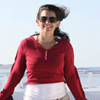
\includegraphics{../pictures/Amanda.jpg}
} &
\raisebox{1in}{\parbox{2.4in}{\textbf{Amanda Lyons --- \textbf{USA}, NY} \textbf{Designer}\textbf{}I am a Visual
Practitioner, Organization Development Consultant \& Experiential
Educator. I love helping people communicate via visual tools that
generally include markers and paper. I think our education system could benefit from using visual communication tools as well as
text based methods. 
%Reach
%\href{https://twitter.com/\#!/amanda\_lyons}{Amanda on Twitter}
%\textbar{} \href{http://www.visualsforchange.com/blog\%20\%20}{Amanda's personal website}
}}
\end{tabular}

\marktransitionempty

\begin{tabular}{lp{2.5in}}
\raisebox{.3in}{
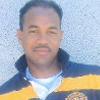
\includegraphics{../pictures/Christopher.jpg}
} &
\raisebox{1in}{\parbox{2.4in}{\textbf{Christopher Neal --- USA, WA} \textbf{(Communications and Media)} I am driven by
technology and its ability to modify virtual communities and social
media, and a passion for Social:Learn, Social:iA, Situated
Cognition, Social Learning Theory, Connectivism, etc. 
%\href{https://plus.google.com/u/0/106960445015668581969/posts}{Christopher
%on Google+} \textbar{}
%\href{http://beyondcredentials.com/index.php?option=com\_bc\_profile\_pages\&uname=berkeleyalum}{Christopher's personal website}
}}
\end{tabular}


\marktransitionempty

\begin{tabular}{lp{2.5in}}
\raisebox{.3in}{
\vspace{-1em}

\includegraphics{../pictures/Ted.jpg}
\vspace{-2em}
} &
\raisebox{1in}{\parbox{2.4in}{\textbf{Ted Newcomb --- USA, AZ} \textbf{(Author, Project Management)} Happily retired grandpa, curating on digital culture,
sociology of the web; interested in collaboration and cooperation in
digital networks that result in positive change.
%\href{http://about.me/tcnewcomb}{Ted on About.me} \textbar{}
%\href{http://www.tcnewcomb.com}{Ted's personal website}
}}
\end{tabular}

\marktransitionempty

\begin{tabular}{lp{2.5in}}
\raisebox{.3in}{
\vspace{-1em}
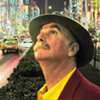
\includegraphics{../pictures/Howard.jpg}
\vspace{-1em}
} &
\raisebox{1in}{\parbox{2.4in}{\textbf{Howard Rheingold --- USA, CA} \textbf{(Author, Editor)} Inspired by
Charles Danoff and Joe Corneli's work on paragogy, I instigated the
Peeragogy project in order to provide a resource for self-organizing
self-learners. Learning is my passion. 
%Reach
%\href{https://twitter.com/\#!/hrheingold}{Howard on Twitter} \textbar{}
%\href{http://www.rheingold.com}{Howard's personal
%website}
}}
\end{tabular}

\marktransitionempty

\begin{tabular}{lp{2.5in}}
\raisebox{.3in}{
\vspace{-1em}

\includegraphics{../pictures/Paola.jpg}
} &
\raisebox{1in}{\parbox{2.4in}{\textbf{Paola Ricaurte --- Mexico} \textbf{(Author)} My believe: education and
technology are essential tools for social change. My challenges:
activist, teacher, mother, immigrant. My philosophy: I am what I am
because of who we all are.
%\href{https://twitter.com/paolaricaurte}{Paola on Twitter} \textbar{}
%\href{http://blogs.eluniversal.com.mx/virtualis/}{Paola's personal
%website}
}}
\end{tabular}

\marktransitionempty

\begin{tabular}{lp{2.5in}}
\raisebox{.3in}{
%\vspace{-1em}
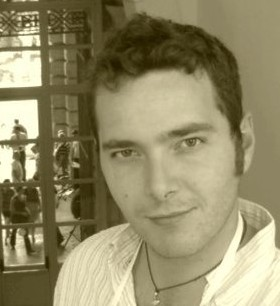
\includegraphics[width=1.4in]{../pictures/fabrizio.jpg}
} &
\raisebox{1in}{\parbox{2.4in}{\textbf{Fabrizio Terzi --- Italy} \textbf{(Inventor, Designer, Translator)} 
I am involved in social and educational projects related to public access to knowledge and cultural diversity. I am an active member of FSF and the FTG -- working on Free Culture.
%\href{http://identi.ca/siar}{Fabrizio on Identica} \textbar{}
%\href{http://theftgacademy.org/}{Fabrizio's personal website}
}}
\end{tabular}

\marktransitionempty

\begin{minipage}{3in}
\textbf{Geoff Walker --- U.K. (Author)} A Further and Higher Education Lecturer
and Tutor, social networker, e-learning advocate. 
%\href{https://twitter.com/\#!/geoffreyawalker}{Geoff on
%Twitter} 
%\textbar{} \href{http://geoffreyawalker.blog.co.uk}{Geoff's personal website}  
\begin{center}
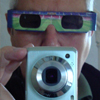
\includegraphics{../pictures/Geoff.jpg}
\end{center}
\end{minipage}
